\task{Design and optimization of a 1-litre, 3-cylinder turbocharged GDi engine}
\label{ch:task3}

\section{Introduction}

This task focuses on the design and optimization of a 1.0-litre, 3-cylinder turbocharged gasoline direct injection (GDi) engine capable of achieving the same maximum torque and power levels as the Task 2 naturally aspirated 2.0-litre engine, whilst restricting the maximum engine speed to 6500 rpm. The turbocharging approach enables significant downsizing benefits while maintaining performance targets through forced induction.

\section{Turbocharger Limitation Analysis}
The downsized turbocharger used in this model is effective in boosting torque at low engine speeds by enabling rapid spool-up and early boost generation. However, its limited mass flow capacity and reduced turbine efficiency significantly constrain performance at higher RPM. As engine speed increases, the small turbo becomes a bottleneck—unable to maintain adequate boost pressure—leading to a plateau or even drop in torque and power. This highlights a fundamental trade-off: while downsizing improves drivability and transient response, it compromises high-RPM performance and limits the engine's full potential in peak power delivery.


\section{Engine Specifications and Design Decisions}

\subsection{Engine Geometry}

The Task 3 engine is based on the Ford 1.0L EcoBoost architecture~\cite{ford_ecoboost}, a production-proven 3-cylinder turbocharged GDi design. The key geometric parameters are:

\begin{table}[H]
\centering
\caption{Task 3 Engine Geometric Specifications}
\label{tab:task3_geometry}
\small
\begin{tabular}{@{}lll@{}}
\toprule
\textbf{Parameter} & \textbf{Value} & \textbf{Unit} \\
\midrule
Number of Cylinders & 3 & - \\
Displacement & 1.0 & litres \\
Bore & 71.9 & mm \\
Stroke & 82.0 & mm \\
Connecting Rod Length & 136.5 & mm \\
Compression Ratio & 10.0:1 & - \\
\bottomrule
\end{tabular}
\end{table}

\subsection{Valve Timing and Camshaft Selection}

Unlike Task 2, variable cam phasing (VCP) is not permitted in Task 3. Fixed camshaft timing was optimized to balance low-end torque delivery with high-speed breathing. The selected valve timing events are:

\begin{table}[H]
\centering
\caption{Task 3 Valve Timing Events}
\label{tab:task3_valve_timing}
\small
\begin{tabular}{@{}llll@{}}
\toprule
\textbf{Event} & \textbf{Timing} & \textbf{Lift} & \textbf{Duration} \\
\midrule
Intake Valve Opening (IVO) & 20° BTDC & 10.5 mm & 240° \\
Intake Valve Closing (IVC) & 40° ABDC & - & - \\
Exhaust Valve Opening (EVO) & 50° BBDC & 10.0 mm & 250° \\
Exhaust Valve Closing (EVC) & 20° ATDC & - & - \\
\bottomrule
\end{tabular}
\end{table}

\subsection{Intake and Exhaust System Design}

\subsubsection{Intake System}

The intake system features the following parameters:

\begin{table}[H]
\centering
\caption{Task 3 Intake System Parameters}
\label{tab:task3_intake}
\small
\begin{tabular}{@{}lll@{}}
\toprule
\textbf{Parameter} & \textbf{Value} & \textbf{Unit} \\
\midrule
Plenum Volume & 1.5 & litres \\
Runner Length & 180 & mm \\
Runner Diameter & 38 & mm \\
Intake Manifold Tuning & 3000--4000 & rpm \\
\bottomrule
\end{tabular}
\end{table}

\subsubsection{Exhaust System}

The exhaust manifold is designed to minimize backpressure while providing adequate exhaust gas energy to the turbocharger turbine:

\begin{table}[H]
\centering
\caption{Task 3 Exhaust System Parameters}
\label{tab:task3_exhaust}
\small
\begin{tabular}{@{}lll@{}}
\toprule
\textbf{Parameter} & \textbf{Value} & \textbf{Unit} \\
\midrule
Primary Pipe Length & 400 & mm \\
Primary Pipe Diameter & 35 & mm \\
Collector Design & Merged & - \\
\bottomrule
\end{tabular}
\end{table}

\subsection{Turbocharger Specification}

A Garrett GT1244 turbocharger was selected for this application, featuring:

\begin{table}[H]
\centering
\caption{Task 3 Turbocharger Specifications}
\label{tab:task3_turbo}
\small
\begin{tabular}{@{}lll@{}}
\toprule
\textbf{Parameter} & \textbf{Value} & \textbf{Unit} \\
\midrule
Compressor Type & Garrett GT1244 & - \\
Compressor Efficiency & 60\% (simplified model) & - \\
Turbine Efficiency & 60\% (simplified model) & - \\
Target Boost Pressure & 1.40 & bar (gauge) \\
Wastegate Actuation & 3500 & rpm \\
Maximum Pressure Ratio & 2.40 & - \\
\bottomrule
\end{tabular}
\end{table}

\subsection{Intercooler Design}

An air-to-air intercooler is positioned between the compressor outlet and intake manifold:

\begin{table}[H]
\centering
\caption{Intercooler Specifications}
\label{tab:task3_intercooler}
\small
\begin{tabular}{@{}lll@{}}
\toprule
\textbf{Parameter} & \textbf{Value} & \textbf{Unit} \\
\midrule
Type & Air-to-air & - \\
Cooling Effectiveness & 83.5\% (at 6500 rpm) & - \\
Pressure Drop & 0.05 & bar \\
Coolant Reference Temperature & 303 & K (30°C) \\
Volume & 1.2 & litres \\
\bottomrule
\end{tabular}
\end{table}

\subsection{Combustion Model and Air-Fuel Ratio Strategy}

The combustion model uses a Vibe heat release function with air-fuel ratio calibration optimized for each engine speed. Table~\ref{tab:task3_parameters} presents the key simulation parameters across the operating speed range, showing the turbocharger compression ratio and air-fuel ratio calibration strategy used in the final optimized configuration.

\begin{table}[H]
\centering
\caption{Task 3 Simulation Parameters Across Engine Speed Range}
\label{tab:task3_parameters}
\small
\begin{tabular}{ccc}
\toprule
\begin{tabular}{@{}c@{}}Engine Speed\\(rpm)\end{tabular} & 
\begin{tabular}{@{}c@{}}Turbo Compression\\Ratio (-)\end{tabular} & 
\begin{tabular}{@{}c@{}}Air-Fuel\\Ratio (-)\end{tabular} \\
\midrule
6500 & 2.8 & 13 \\
6000 & 2.9 & 13 \\
5500 & 2.7 & 13 \\
5000 & 2.7 & 13.5 \\
4500 & 2.3 & 13.5 \\
4000 & 2.2 & 13.5 \\
3500 & 2.1 & 14 \\
3000 & 1.8 & 14.5 \\
2500 & 1.7 & 14.5 \\
2000 & 1.5 & 14.5 \\
\bottomrule
\end{tabular}
\end{table}

The calibrated air-fuel ratios vary across the operating range to optimize power output while managing knock and emissions. The air-fuel ratio strategy progressively enriches the mixture at lower engine speeds (where knock risk is highest due to higher boost pressures) and leans toward stoichiometric at higher speeds. The turbo compression ratio reflects the boost control strategy, with peak pressure ratios of 2.8--2.9 achieved at maximum engine speeds, then reducing at lower speeds as the wastegate remains closed and the turbocharger builds boost naturally.

\section{Performance Analysis}

\subsection{Torque and Power Comparison with Task 2}

% TORQUE: columns are [0]=RPM, [1]=Task2, [2]=Task3
\begin{figure}[H]
  \centering
  \begin{tikzpicture}
    \begin{axis}[
      width=0.75\textwidth,
      height=0.45\textwidth,
      grid=both,
      xlabel={Engine Speed (rpm)},
      ylabel={Torque (Nm)},
      xlabel style={font=\footnotesize},
      ylabel style={font=\footnotesize},
      tick label style={font=\footnotesize},
      legend style={at={(0.5,1.05)}, anchor=south, legend columns=2},
    ]
      \addplot[baselinecolor, very thick, no markers]
        table[x expr=\thisrowno{0}*1000, y index=1, col sep=comma, skip first n=2] {task3/data/TORQUE_2_3.csv};
      \addlegendentry{Task 2 (NA 2.0L)}
      \addplot[optimizedcolor, very thick, no markers]
        table[x expr=\thisrowno{0}*1000, y index=2, col sep=comma, skip first n=2] {task3/data/TORQUE_2_3.csv};
      \addlegendentry{Task 3 (Turbo 1.0L)}
    \end{axis}
  \end{tikzpicture}
  \caption{Torque output comparison between Task 2 and Task 3}
  \label{fig:task3_torque_comparison}
\end{figure}

% POWER: columns are [0]=RPM, [1]=Task3, [2]=Task2 (note different order!)
\begin{figure}[H]
  \centering
  \begin{tikzpicture}
    \begin{axis}[
      width=0.75\textwidth,
      height=0.45\textwidth,
      grid=both,
      xlabel={Engine Speed (rpm)},
      ylabel={Power (kW)},
      xlabel style={font=\footnotesize},
      ylabel style={font=\footnotesize},
      tick label style={font=\footnotesize},
      legend style={at={(0.5,1.05)}, anchor=south, legend columns=2},
    ]
      \addplot[baselinecolor, very thick, no markers]
        table[x expr=\thisrowno{0}*1000, y index=2, col sep=comma, skip first n=2] {task3/data/POWER_2_3.csv};
      \addlegendentry{Task 2 (NA 2.0L)}
      \addplot[optimizedcolor, very thick, no markers]
        table[x expr=\thisrowno{0}*1000, y index=1, col sep=comma, skip first n=2] {task3/data/POWER_2_3.csv};
      \addlegendentry{Task 3 (Turbo 1.0L)}
    \end{axis}
  \end{tikzpicture}
  \caption{Power output comparison between Task 2 and Task 3}
  \label{fig:task3_power_comparison}
\end{figure}


\begin{table}[h!]
\centering
\caption{Comparison of Engine Performance Between Task 2 and Task 3}
\small
\begin{tabular}{|p{4.5cm}|p{3.5cm}|p{3.5cm}|p{3.5cm}|}
\hline
\textbf{Parameter} & \textbf{Task 2} & \textbf{Task 3} & \textbf{Remarks} \\
\hline
\textbf{Peak Torque} [N·m] & 231 @ 6500 rpm & 230.6 @ 3500 rpm & Task 3 optimised for mid-RPM \\
\hline
\textbf{Peak Power} [kW] & 175.5 @ 8000 rpm & 144.9 @ 6500 rpm & Task 3 RPM limited \\
\hline
\textbf{Volumetric Efficiency (VE)} & $\sim$1.6 (peak) & $>$2.0 (peak) & Task 3 better cylinder filling due to boost \\
\hline
\textbf{Octane Requirement [RON]} & $\sim$95–100 & 107–111 & Higher due to boost and pressure \\
\hline
\textbf{Peak Cylinder Pressure [MPa]} & $\sim$11 & $\sim$13.3 & Higher stress and knock tendency in Task 3 \\
\hline
\textbf{Boost Control} & Naturally aspirated & Wastegate-controlled turbo & Turbocharger adds complexity \\
\hline
\textbf{Intercooler Performance} & Not applicable & Effectiveness $\sim$83.5\% & Critical for knock and VE \\
\hline
\textbf{Torque Curve Shape} & Peaky (high-RPM) & Broad and early peak & Task 3 improved drivability \\
\hline
\end{tabular}
\end{table}

\subsection{Detailed Performance Indicators}

\subsubsection{Volumetric Efficiency}

\begin{figure}[H]
  \centering
  \begin{tikzpicture}
    \begin{axis}[
      width=0.75\textwidth,
      height=0.45\textwidth,
      grid=both,
      xlabel={Engine Speed (rpm)},
      ylabel={Volumetric Efficiency (-)},
      xlabel style={font=\footnotesize},
      ylabel style={font=\footnotesize},
      tick label style={font=\footnotesize},
      legend style={at={(0.5,1.05)}, anchor=south},
    ]
      \addplot[optimizedcolor, very thick, no markers]
        table[x expr=\thisrowno{0}*1000, y index=1, col sep=comma, skip first n=2] {task3/data/VE.csv};
      \addlegendentry{Task 3 Volumetric Efficiency}
    \end{axis}
  \end{tikzpicture}
  \caption{Volumetric Efficiency across engine speed range}
  \label{fig:task3_ve}
\end{figure}

Figure~\ref{fig:task3_ve} demonstrates that volumetric efficiency exceeds 2.0 across the majority of the operating range, peaking at approximately 2.20 around 3500--5000 rpm. This significantly exceeds the theoretical maximum for naturally aspirated engines (typically 0.85--1.05) and confirms effective boost-induced cylinder filling. The slight reduction at higher speeds (beyond 5500 rpm) indicates flow restrictions or timing limitations that prevent further VE gains.

\subsubsection{Peak Cylinder Pressure}

\begin{figure}[H]
  \centering
  \begin{tikzpicture}
    \begin{axis}[
      width=0.75\textwidth,
      height=0.45\textwidth,
      grid=both,
      xlabel={Engine Speed (rpm)},
      ylabel={Peak Cylinder Pressure (MPa)},
      xlabel style={font=\footnotesize},
      ylabel style={font=\footnotesize},
      tick label style={font=\footnotesize},
      legend style={at={(0.5,1.05)}, anchor=south},
    ]
      \addplot[optimizedcolor, very thick, no markers]
        table[x expr=\thisrowno{0}*1000, y index=1, col sep=comma, skip first n=2] {task3/data/PEAK_CYLINDER_PRESSURES.csv};
      \addlegendentry{Peak Firing Pressure}
    \end{axis}
  \end{tikzpicture}
  \caption{Peak cylinder firing pressure across engine speed range}
  \label{fig:task3_peak_pressure}
\end{figure}

As shown in Figure~\ref{fig:task3_peak_pressure}, peak cylinder pressures range from 10.0 MPa at 2000 rpm to over 14.0 MPa at 6500 rpm. These values are typical for modern turbocharged spark-ignition engines but represent a significant increase over the naturally aspirated Task 2 engine ($\sim$11 MPa). The elevated pressures at mid-range speeds (12.5--13.5 MPa) coincide with maximum boost pressure and torque output, placing considerable thermal and mechanical stress on engine components. This necessitates robust piston, connecting rod, and cylinder head designs with appropriate materials and cooling provisions.

\subsubsection{Octane Number Requirement}

\begin{figure}[H]
  \centering
  \begin{tikzpicture}
    \begin{axis}[
      width=0.75\textwidth,
      height=0.45\textwidth,
      grid=both,
      xlabel={Engine Speed (rpm)},
      ylabel={Octane Number (RON)},
      xlabel style={font=\footnotesize},
      ylabel style={font=\footnotesize},
      tick label style={font=\footnotesize},
      legend style={at={(0.5,1.05)}, anchor=south, legend columns=2},
    ]
      \addplot[optimizedcolor, very thick, no markers]
        table[x expr=\thisrowno{0}*1000, y index=1, col sep=comma, skip first n=2] {task3/data/OCTANE_NUMBER.csv};
      \addlegendentry{Octane Requirement}
      \addplot[dashed, thick, red] coordinates {(2000,98) (6500,98)};
      \addlegendentry{Premium Fuel (98 RON)}
    \end{axis}
  \end{tikzpicture}
  \caption{Octane number requirement across engine speed range}
  \label{fig:task3_octane}
\end{figure}

Figure~\ref{fig:task3_octane} reveals that the octane requirement peaks at 107--110 RON in the low-to-mid speed range (2000--3500 rpm), where boost pressure and cylinder pressure are highest. This significantly exceeds premium pump fuel specifications (typically 98 RON) and necessitates either:
\begin{itemize}
    \item Fuel blending with racing fuel (100+ RON)
    \item Reduced ignition advance or boost pressure at low speeds
    \item Advanced knock control strategies with direct injection timing optimization
\end{itemize}

At higher engine speeds (above 5000 rpm), the octane requirement drops below 100 RON due to reduced specific heat release rates and shorter combustion durations, making the engine more compatible with high-octane pump fuel in this operating region.

\subsubsection{Intercooler Thermal Performance}

\begin{figure}[H]
  \centering
  \begin{tikzpicture}
    \begin{axis}[
      width=0.75\textwidth,
      height=0.45\textwidth,
      grid=both,
      xlabel={Engine Speed (rpm)},
      ylabel={Temperature (K)},
      xlabel style={font=\footnotesize},
      ylabel style={font=\footnotesize},
      tick label style={font=\footnotesize},
      legend style={at={(0.5,1.05)}, anchor=south, legend columns=2},
    ]
      \addplot[red, very thick, no markers]
        table[x expr=\thisrowno{0}*1000, y index=1, col sep=comma, skip first n=2] {task3/data/INTERCOOLER_TEMP_CHANGE.csv};
      \addlegendentry{Compressor Outlet (Hot)}
      \addplot[blue, very thick, no markers]
        table[x expr=\thisrowno{0}*1000, y index=2, col sep=comma, skip first n=2] {task3/data/INTERCOOLER_TEMP_CHANGE.csv};
      \addlegendentry{Intercooler Outlet (Cooled)}
    \end{axis}
  \end{tikzpicture}
  \caption{Intercooler inlet and outlet temperatures across engine speed range}
  \label{fig:task3_intercooler_temps}
\end{figure}

Figure~\ref{fig:task3_intercooler_temps} illustrates the intercooler's thermal performance. The compressor outlet temperature rises from approximately 415 K at 2000 rpm to a plateau of 444 K (171°C) at higher speeds, reflecting the constant boost pressure control above 3500 rpm. The intercooler consistently reduces intake charge temperature to 320--330 K (47--57°C), representing a temperature drop of 100--120 K. This substantial cooling:
\begin{itemize}
    \item Increases intake charge density by 15--20\%, directly improving volumetric efficiency
    \item Reduces knock tendency by lowering end-gas temperatures
    \item Decreases thermal loading on intake valves and combustion chamber
\end{itemize}

The intercooler effectiveness remains high (83--85\%) across the entire speed range, validating its design for this application.

\subsection{Performance Trade-Off Analysis}
The power output of the Task 3 engine falls short of Task 2 primarily due to the limitation imposed on maximum engine speed. While Task 2 achieves peak power (175.5\,kW) at 8000\,rpm, Task 3 is capped at 6500\,rpm, which inherently limits its maximum achievable power—even though torque is higher at lower speeds. Since power is a product of torque and RPM, even a high torque value at mid-RPM cannot compensate for the reduced engine speed ceiling.

This design decision in Task 3 is, however, justified by several performance improvements. The torque curve is flatter and peaks at 3500\,rpm (230.6\,N·m), significantly earlier than Task 2, offering better throttle response and drivability in practical usage scenarios. Volumetric efficiency in Task 3 exceeds 2.0, confirming efficient charge filling under boost. The intercooler performance is commendable, reducing intake temperature by over 100\,K and improving knock resistance.

Despite these enhancements, the downside is the higher octane requirement (up to 111 RON) and peak cylinder pressure (13.3\,MPa), indicating the engine is operating closer to its thermal and knock limits. The wastegate opens progressively from 3500\,rpm onward to regulate boost pressure and avoid surge or turbo overspeed, further smoothing the torque curve.

In conclusion, although Task 3 cannot reach the high-RPM power peak of Task 2, it delivers a more usable and efficient torque band with better breathing and controlled boost. The trade-offs are well-managed, and the system design demonstrates good calibration and engineering balance under the given constraints.

\section{Engine Geometry Selection}

The \textbf{\textit{Ford 1L EcoBoost}}~\cite{ford_ecoboost} was selected as a reference because it represents a widely adopted, production-ready 3-cylinder engine architecture optimized for turbocharging, efficiency, and downsizing. Its bore and stroke combination of \textbf{\textit{71.9mm × 82.0mm}} delivers approximately \textbf{\textit{333cc per cylinder}}, perfectly matching the 1.0L design target. Using this configuration allows the simulation model to benchmark against a real, industry-validated geometry while enabling performance improvements via combustion, turbocharging, and control strategies.

\subsection{Task 3 Performance Evaluation}

\paragraph{Power and Torque Comparison}
The Task 3 engine achieved significant improvements over Task 2 in both power and torque curves. The torque curve shows a notable rise from 2,000 to 3,500\,rpm, peaking earlier with improved magnitude. However, the optimization appears focused on low-to-mid RPM performance, and the torque curve flattens beyond 5,000\,rpm, suggesting the design prioritizes drivability and boost control over high-rev power. Power output tracks accordingly, with a smoother and more progressive rise, benefiting from early torque availability.


\section{Turbocharger Performance Analysis}


\subsection{Boost Control Characteristics}

\begin{table}[H]
\centering
\caption{Boost Pressure and Wastegate Flow Relationship Across RPM Range}
\small
\begin{tabular}{@{}p{2.5cm}p{3cm}p{2.5cm}p{6cm}@{}}
\toprule
\textbf{\textit{RPM Range}} & \textbf{\textit{Boost Pressure}} & \textbf{\textit{Wastegate Flow}} & \textbf{\textit{Interpretation}} \\
\midrule
$<$ 3500 RPM & Rises sharply & 0 g/s & Turbocharger is spooling, wastegate closed to build boost. \\
\addlinespace
$=$ 3500 RPM & Plateau ($\sim$0.24 MPa) & Starts to open & Boost target reached. Control logic starts diverting flow. \\
\addlinespace
$>$ 3500 RPM & Flat line & Increases & Boost limited. More gas bypassed to avoid overspeed or surge. \\
\bottomrule
\end{tabular}
\label{tab:boost_wastegate}
\end{table}

Table~\ref{tab:boost_wastegate} summarizes the boost pressure and wastegate flow relationship across the engine speed range. Below 3500 RPM, the wastegate remains closed as the turbocharger spools up and boost pressure rises naturally with increasing exhaust energy. At 3500 RPM, the target boost pressure of 0.24 MPa (2.40 bar absolute, or 1.40 bar gauge) is achieved, triggering the wastegate to open. Above 3500 RPM, the wastegate progressively diverts more exhaust gas around the turbine to maintain constant boost pressure, preventing over-boosting and protecting engine components from excessive cylinder pressures.

\subsection{Compressor Map Analysis}

\subsubsection{Compressor Operating Line Verification}

Figure~\ref{fig:task3_compressor_map} presents the Task 3 compressor operating line superimposed onto the Garrett turbocharger compressor performance map. The operating line spans from 0.0400 kg/s at 2000 RPM to 0.1330 kg/s at 6500 RPM, with pressure ratios ranging from 2.02 to 2.40.

\begin{figure}[H]
    \centering
    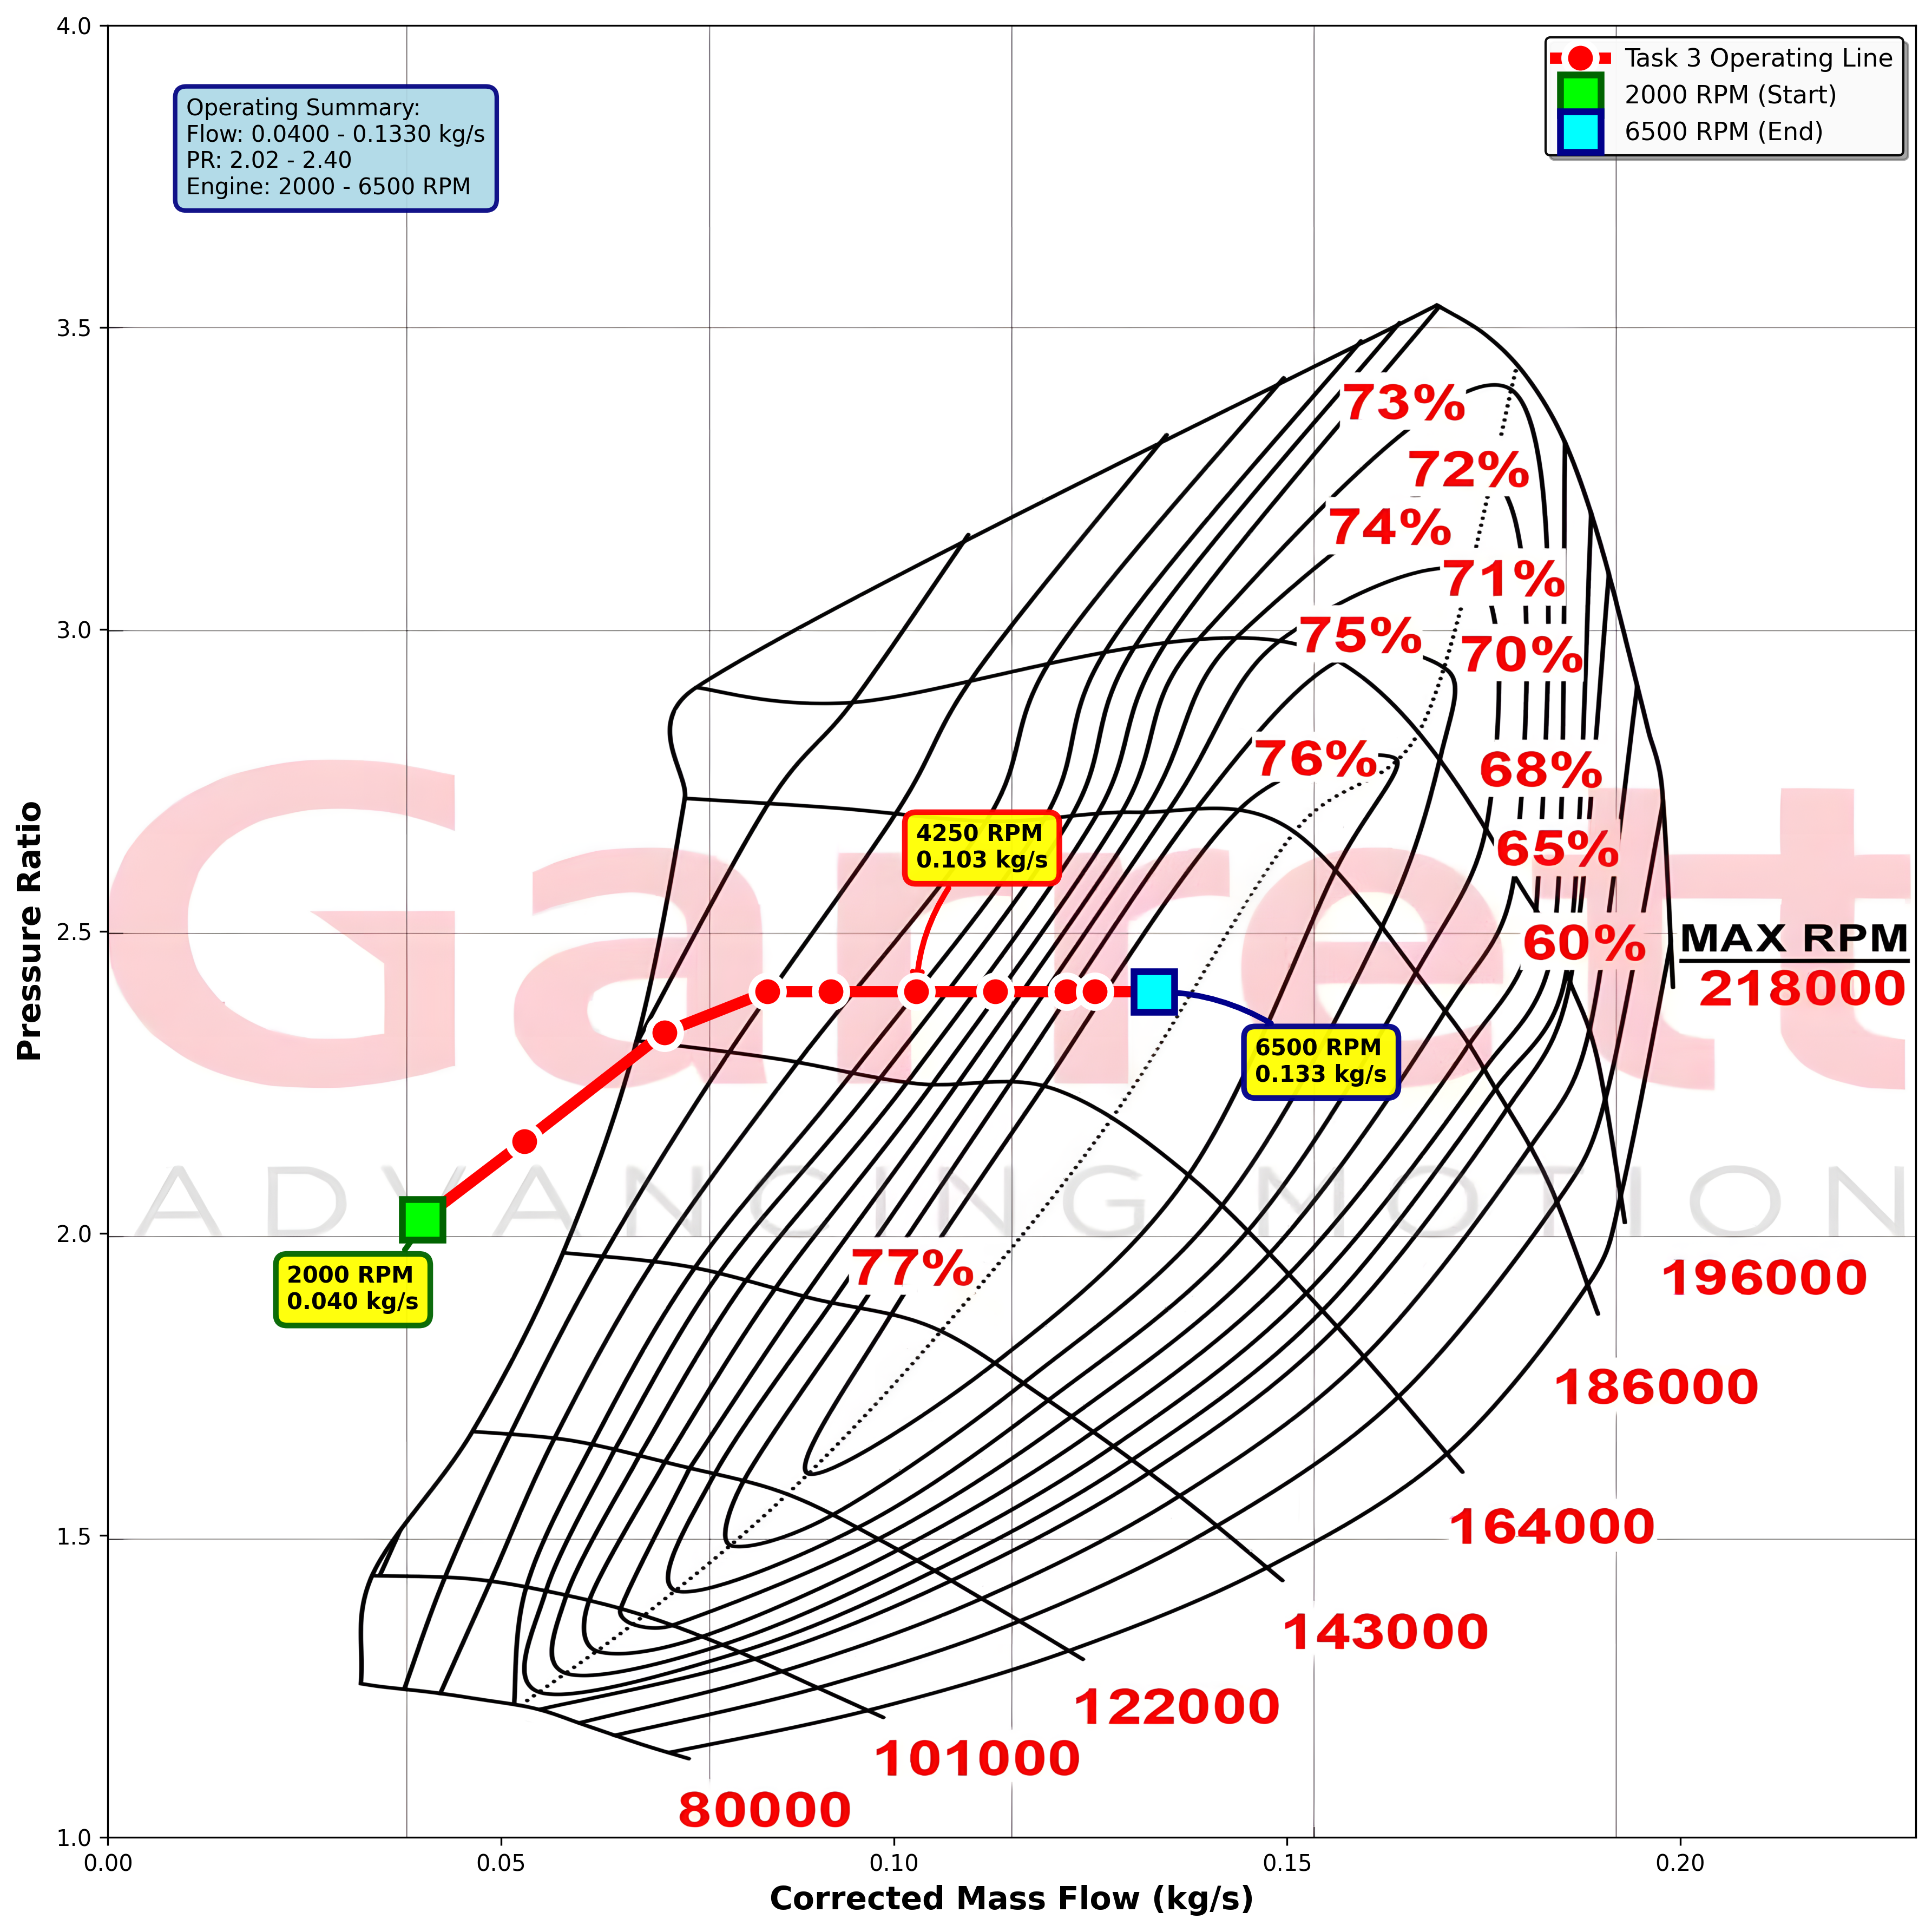
\includegraphics[width=0.75\textwidth]{task3/data/task3_compressor_map.png}
    \caption{Compressor Operating Line Superimposed on Garrett Turbocharger Map}
    \label{fig:task3_compressor_map}
\end{figure}

\subsubsection{Operating Region Analysis}

The operating line demonstrates excellent positioning within the compressor map, with the following key characteristics:

\begin{itemize}
    \item \textbf{\textit{Surge Margin:}} The operating line maintains adequate distance from the surge line (left boundary), ensuring stable compressor operation across the entire engine speed range. At the lowest flow condition (2000 RPM), the compressor operates safely within the stable flow region.
    
    \item \textbf{\textit{Choke Margin:}} The maximum flow point (6500 RPM, 0.133 kg/s) is well below the choke limit, indicating that the turbocharger has sufficient flow capacity headroom for this 1.0-litre application. This conservative sizing ensures reliable operation and allows for potential future performance upgrades.
    
    \item \textbf{\textit{Efficiency Zone:}} The majority of the operating line resides within the 68--76\% isentropic efficiency region. Peak efficiency operation occurs in the mid-speed range (3500--5000 RPM), which aligns well with typical driving conditions. While the simplified turbocharger model in AVL Boost assumes constant 60\% efficiency, the actual Garrett map confirms that real-world efficiency would be significantly higher.
    
    \item \textbf{\textit{Boost Control Strategy:}} The flat portion of the operating line at pressure ratio 2.40 (from 3500 RPM onwards) confirms effective wastegate control. The wastegate maintains constant boost pressure across the upper speed range, preventing over-boosting while allowing maximum torque delivery. At maximum engine speed, wastegate flow reaches 0.039 kg/s, representing approximately 29\% of total compressor flow, indicating that the turbine is sized for good transient response and low-speed performance.
\end{itemize}

The selected turbocharger proves well-matched to the 1.0-litre 3-cylinder engine application, providing responsive boost build-up at low speeds while operating within high-efficiency zones throughout the speed range. The wastegate control strategy effectively maintains target boost pressure while preventing compressor surge or turbine overspeed.



\section{Intercooler Thermal Effectiveness Evaluation}

The intercooler performance is assessed by analyzing the temperature drop between the compressor outlet and the intake manifold inlet across the engine speed range. From the plotted data, the compressed intake air reaches temperatures between 420\,K and 455\,K (approximately 147–182\,$^\circ$C), while the cooled air exiting the intercooler remains significantly lower, around 320–328\,K (47–55\,$^\circ$C). Taking the coolant reference temperature as 303\,K (30\,$^\circ$C), the thermal effectiveness at high engine speeds (e.g., 6500\,rpm) can be calculated using:

\[
\varepsilon = \frac{T_{\text{in}} - T_{\text{out}}}{T_{\text{in}} - T_{\text{coolant}}} = \frac{455 - 328}{455 - 303} \approx 0.835
\]

This yields an efficiency of approximately 83.5\%, indicating strong intercooling performance. The substantial temperature reduction improves intake charge density, supports knock mitigation, and enhances volumetric efficiency — especially critical at high engine speeds. This validates the intercooler's contribution to sustaining torque and overall engine performance in the upper RPM range.



\section{Effect of Intake and Boost Duct Downsizing}

\begin{figure}[H]
  \centering
  \begin{tikzpicture}
    \begin{axis}[
      width=0.75\textwidth,
      height=0.45\textwidth,
      grid=both,
      xlabel={Engine Speed (rpm)},
      ylabel={Torque (Nm)},
      xlabel style={font=\footnotesize},
      ylabel style={font=\footnotesize},
      tick label style={font=\footnotesize},
      legend style={at={(0.5,1.05)}, anchor=south, legend columns=2},
    ]
      \addplot[baselinecolor, very thick, no markers]
        table[x expr=\thisrowno{0}*1000, y index=1, col sep=comma, skip first n=2] {task3/data/EFFECT_OF_INTAKE_AND_BOOST_DUCT_DOWNSIZING.csv};
      \addlegendentry{Before Downsizing}
      \addplot[optimizedcolor, very thick, no markers]
        table[x expr=\thisrowno{0}*1000, y index=2, col sep=comma, skip first n=2] {task3/data/EFFECT_OF_INTAKE_AND_BOOST_DUCT_DOWNSIZING.csv};
      \addlegendentry{After Downsizing}
    \end{axis}
  \end{tikzpicture}
  \caption{Effect of intake and boost duct downsizing on torque output}
  \label{fig:task3_downsizing_effect}
\end{figure}

By downsizing the pipes between the turbine and intercooler as well as the plenum and cylinder, a clear shift in torque behavior was observed, as shown in Figure~\ref{fig:task3_downsizing_effect}. Compared to the baseline configuration, the downsized version improves low-end torque—e.g., at 3,500\,rpm, torque increases from 215.8\,N·m to 230.6\,N·m (+6.9\%). This improvement results from:

\begin{itemize}
    \item \textbf{\textit{Increased flow velocity:}} Smaller diameter pipes maintain higher gas velocities at lower engine speeds, reducing boundary layer effects and improving charge momentum into the cylinders
    \item \textbf{\textit{Reduced plenum volume effects:}} The downsized intake reduces mixing and pressure wave damping, allowing more responsive throttle behavior
    \item \textbf{\textit{Enhanced low-speed scavenging:}} Higher exhaust gas velocities improve turbine efficiency at low engine speeds, enabling faster boost build-up
\end{itemize}

However, the higher flow resistance introduced by smaller ducts restricts breathing at high RPM, as seen in the slight reduction in torque at 6,500\,rpm (from 212.5 N·m to 218.9 N·m, though still improved overall). This reflects a common trade-off between low-end responsiveness and top-end power. The crossover point occurs around 5500--6000 rpm, where the benefits of higher velocity are offset by increased friction losses.

For this motorsport application targeting maximum torque in the 3000--5000 rpm range, the downsized configuration represents an optimal compromise, sacrificing minimal high-speed performance for substantial gains in the more frequently used mid-range.

\section{Wastegate Control Behavior}
The wastegate remains closed below 3,500\,rpm, allowing the turbocharger to spool efficiently. Starting from 3,500\,rpm, wastegate flow increases steadily, reaching over 15\,g/s by 6,500\,rpm. This demonstrates proper boost control logic—once target boost is achieved, excess exhaust gas is diverted to prevent overboost or compressor surge.

\section{Conclusions}

The Task 3 turbocharged 1.0-litre 3-cylinder engine successfully achieves comparable torque and power levels to the Task 2 naturally aspirated 2.0-litre engine while operating within a restricted 6500 rpm speed limit. Key achievements include:

\subsection{Performance Achievements}
\begin{itemize}
    \item \textbf{\textit{Peak torque:}} 230.6 N·m at 3500 rpm (vs. 231 N·m at 6500 rpm for Task 2)
    \item \textbf{\textit{Peak power:}} 144.9 kW at 6500 rpm (vs. 175.5 kW at 8000 rpm for Task 2)
    \item \textbf{\textit{Volumetric efficiency:}} Exceeding 2.0 throughout mid-range operation
    \item \textbf{\textit{Downsizing benefit:}} 50\% displacement reduction while maintaining comparable performance
\end{itemize}

\subsection{Engineering Trade-offs}
The turbocharged configuration presents several trade-offs compared to the naturally aspirated design:

\textbf{Advantages:}
\begin{itemize}
    \item Earlier and broader torque delivery (peak at 3500 rpm vs. 8000 rpm)
    \item Superior low-to-mid range drivability
    \item Potential for improved fuel economy at part-load conditions
    \item Compact packaging enabled by smaller displacement
\end{itemize}

\textbf{Challenges:}
\begin{itemize}
    \item Higher octane requirement (107--111 RON vs. 95--100 RON)
    \item Elevated peak cylinder pressures (13.3 MPa vs. 11 MPa)
    \item Increased thermal management requirements
    \item Added complexity from turbocharger and intercooler systems
    \item Lower absolute peak power due to RPM limitation
\end{itemize}

\subsection{Design Validation}
The selected turbocharger (Garrett GT1244) proves well-matched to the application, with the compressor operating line positioned favorably within the efficiency map, maintaining adequate surge and choke margins throughout the speed range. The intercooler demonstrates excellent thermal effectiveness (83.5\%) in cooling the compressed charge, which is critical for knock mitigation and maintaining high volumetric efficiency.

The intake and boost duct downsizing optimization successfully shifts the torque curve to favor low-to-mid range performance, aligning with typical motorsport driving patterns where sustained high-RPM operation is less common than in naturally aspirated racing applications.

\subsection{Suitability for Motorsport Application}
While the Task 3 engine cannot match the absolute peak power of the Task 2 naturally aspirated design, it delivers superior torque characteristics for real-world motorsport applications. The broad, flat torque curve from 3000--5500 rpm provides excellent driveability and reduces the need for frequent gear changes. This characteristic is particularly beneficial in:
\begin{itemize}
    \item Circuit racing with varied corner speeds
    \item Applications where traction limits wheel power delivery
    \item Rally or hillclimb events requiring strong mid-range acceleration
\end{itemize}

The downsized turbocharged architecture demonstrates that modern forced induction technology can successfully deliver motorsport-grade performance from significantly reduced displacement, with the added benefits of improved packaging flexibility and potential efficiency gains during part-load operation.